\documentclass[twoside,11pt]{article}

\usepackage{amssymb,amsmath, mathtools} 
\usepackage{geometry, graphicx}
\usepackage{tabulary}
\usepackage{upgreek}
\usepackage{siunitx}
\usepackage{caption}
\usepackage{subcaption}
\usepackage{csvsimple}
\usepackage{hanging}
\usepackage[export]{adjustbox}
\usepackage{multirow}
\usepackage{url}

\usepackage{enumitem}
\usepackage{physics}

\usepackage{mathtools}

\usepackage{soul}

\newtagform{Eq}{(Equation }{)}
\usetagform{Eq}

\graphicspath{ {../images} }    


\DeclareMathAlphabet{\mathpzc}{OT1}{pzc}{m}{it}
\DeclareMathOperator*{\argmax}{arg\,max}
\DeclareMathOperator*{\argmin}{arg\,min}


\usepackage{jmlr2e}

\usepackage[noabbrev,capitalize]{cleveref}



% Heading arguments are {volume}{year}{pages}{submitted}{published}{author-full-names}


% Short headings should be running head and authors' last names


\ShortHeadings{Dissertation Critique}{Jardee}
\firstpageno{1}


\begin{document}


\title{Critique of \ul{Right for the Right Reasons: Training Neural Networks to be Interpretable, Robust, and Consistent with Expert Knowledge}}

\author{\name William Jardee\email willjardee@gmail.com \\
       \addr Physics\\
       Montana State University\\
       Bozeman, MT 59715, USA
       }
\editor{\,}

\maketitle

\begin{abstract}%
% don't forget your abstract dumbass
\end{abstract}
 
\section{Introduction}
Andrew Salvin Ross's doctoral thesis, \ul{Right for the Right Reasons: Training Neural Networks to be Interpretable, Robust, and Consistent with Expert Knowledge} attempts to tackle exactly what the name implies: interpretable neural networks\footnote{The majority of the information provided in this piece is derived from and centered around this thesis. It can be assumed that any statements given are consistent, to my best knowledge, with the thesis unless otherwise stated.}. This topic is motivated by a couple of stories at the beginning, one of which I will summarize. 

A network is attempting to learn individuals that should receive priority emergency care. The performance against the validation sets is consistent, and the model seems to have learned the situation well. Upon closer inspection, the model had learned the rule ``\textit{HasAsthma}$(x) \rightarrow$ \textit{Lower-Risk}$(x)$". Intuitively, this is the opposite of the truth, so what went wrong? In the real-world data, asthmatic patients were automatically given emergency treatment and, consequently, had a higher survival rate. This was not considered in the development of the model, so if it were rolled out, the model would have advised against aiding the patients most at risk. 

These problems motivate the thesis to tackle a) a loss function that accounts for interpretable reasons and b) exploring interpretable representations, described as practical explainability. The former focuses on the theoretical derivation of an input gradient-based approach to qualifying a ``Reason". Once a convincing argument is given, they shift to searching this reason-space for alternative models. An application of this loss function is provided in the context of adversarial neural networks. The defense of this application is that wrong reasons can be thought of as adversarial models embedded in the data. If the proposed model can effectively handle the adversarial context, it should also be able to take misleading patterns in the data.

The second focus of the paper is on how to explain these reasons to humans. This is done through smaller ``Think-aloud" tests and a more extensive test that quantifies the understanding of subjects after interacting with model representations. The paper concludes with a discussion on how to approach hierarchical disentanglement. Hierarchical disentanglement deviates from the concept that low-level features should describe the reasons in a model; instead, they are characterized by a hierarchy of abstract, complex, implicit rules. The author proposes describing the underlying reasons in these networks as a hierarchical tree. 

The rest of this critique will be separated, similar to the structure given in the thesis. In Section~\ref{sec:related works} we describe the relevant background knowledge required through the rest of this critique, as well as briefly touching on some of the inspirations that are behind the paper. Section~\ref{sec:RRR alg} outlines what is Part II of the thesis, which is the theoretical derivation of their crucial algorithm. In Section~\ref{sec:alg exp} the experimental testing of the algorithm is outlined and touches on the application of the algorithm to the adversarial context. Section~\ref{sec:explainability} describes the attempt to create an explainable representation of neural network reasons as well a summary of the hierarchical tree method. Some of the discussions will be scattered throughout. Still, for clarity, the bulk will be collected at the end of Section~\ref{sec:contributions}, with a summary of the contributions of the paper and a quick analysis of them. 

%---------------------------------------------------------------------

\section{Related Works}
\label{sec:related works}
The breadth of this paper includes many examples of algorithms, application settings, and theoretical bases beyond the scope of this critique. For this reason, the extent of related works will be limited to the directly relevant concepts.
\subsection{Explainable Models}
Classifiers sort inputs according to the underlying characteristics learned from training data. It is often assumed, as they do in this thesis, that there exists a set of underlying \textbf{implicit decision rules} that define the function $\vb{X} \rightarrow y$ (input to output class). An \textit{interpretable} model means that these rules provide explanations in forms that humans could understand. There is a distinction between \textit{completely interpretable}, meaning that a human can completely understand the rules, and \textit{completely uninterpreatbale}, where the rules are so complex a human can not completely understand them. The line between the two is tough to characterize, and many problems may be only partially interpretable. 

Machine learning models that attempt to learn explainable models are not a new idea. A common pursuit is using counter-factual explanations, characterizing models by seeing how a small perturbation of the input changes the expected output \citep{2016:lungberg}. An example of a counter-factual model that does not rely on domain-specific details is the LIME (Local Interpretable Model-agnostic Explanations) algorithm \citep{2016:Ribeioro}. The core of LIME is presenting \underline{locally sparse} models of how predictions change with small perturbations of the input. The world of SVMs use linear decision boundaries and sometimes input gradients to provide explanations while optimizing correctness \citep{2007:zaidan}. According to Ross, which seems consistent with a quick search, there are no matured algorithms that consider correctness without relying on being tailored to a domain-specific context. 

\subsection{Ensemble and Adversarial Methods}
Ensembles and adversarial methods can be used to improve the performance of stand-alone models. Ensembling is a helpful tool as it enforces good algorithms with robustness, as it is much less likely that multiple models will give the wrong answer than a single model. An important characteristic in ensemble learning is diversity, as recombining different models is essential to the concept. Some models introduce diversity by a stochastic process, i.e., training on different training sets \citep{breiman2001random}, and some explicitly introduce diversity by encouraging models to specialize in different subsets of the input space \citep{zhou2018diverse}. 

A natural extension of the idea of ensembling is adversarial methods. By developing two models in parallel, one learning to solve the problem, called the defense, and one learning to create erroneous data, called the attack, the resulting model is robust to the most challenging characteristics in the data. Modern adversarial methods, such as the FGSM (Fast Gradient Sign Method) \citep{goodfellow2014generative} and TGSM (Targeted Gradient Sign Method) \citep{kurakin2016adversarial} are built off of a small perturbation of input values by the gradient of the correct response to another possible result. These methods are built off input gradients, the same value that defines the thesis's loss function; thus, it is a reasonable extension of their work.

\subsection{Human Centered Interpretability Measures}
Measuring how interpretable a model is is a difficult task. There is a lot of criticism that the topic is not being well defined \citep{lipton2018mythos} and the metrics for analyzing interpretability are not fully convincing. Consequently, a mixture of qualitative and quantitative methods should be used to explain how compatible humans and AI are. An example of qualitative analysis is ``think-aloud" tests \citep{lewis1982using} and for quantitative analysis: accuracy, speed, and completion. Interpretability is often thought of as manifesting in simulability, an individual's ability to accurately describe the model's interaction with new conditions \citep{miller2019explanation}. 

Representation learning, a common approach to conveying interpretable models, focuses on taking high-dimensional instances and representing them as low-dimensional ones. One approach is disentanglement, where high-dimensional data is mapped to low-dimensional representations such that the new representation's dimensions correspond to ground-truth factors that generate the information \citep{bengio2013representation}. Presenting these representations is a difficult challenge. Some works attempt to show the results of linearly varying values along a particular dimension of the disentanglement \textbf{113, 93, 46, 45, 110} or by small perturbations, as described earlier. A less common but compelling method is with an interactive interface. Exposure to how outputs vary according to specific inputs via slides or discrete modes can quickly provide information but requires the development of such a representation. There is literature exploring the use of sliders \textbf{84} and exemplar models \textbf{168, 169, 9}, where specific dimensions are maximized and minimized to show the range of their impact to describe the effect of selected features. According to Ross, there are not any general methods that can generate baseline characteristics that would be included in these visual representations, let alone generate them automatically.

\subsection{Interpretable Representations}
In the realm of disentanglement, recently, there has been a focus on flat factored representations. The premise of this idea is that the dimensions taken from disentanglement can be understood as independent rules that describe a flat decision space. Assuming that the correct understanding of a model as a whole is a complex rule that considers a combination of lesser decision rules, these factors can help describe a type of hierarchy. It is proposed that this hierarchy is more natural to humans and, consequently, easier to understand.

%---------------------------------------------------------------------

\section{Right for the Right Reasons Algorithm}
\label{sec:RRR alg}
The first novel idea introduced by the paper is a loss function that discourages the impact of gradients in regions declared by a ``annotation" matrix, $A$. This loss function is presented in the context of neural networks. It is pointed out that all of the functions provided are differentiable and thus can be minimized with gradient methods. The first proposed iteration of the process is 
\begin{align}
\mathcal{L}(\theta, \vb{X}, y, A) &  = \underbrace{\sum^N_{n=1}\sum^K_{k=1}-y_{nk}\,\log(\hat{y}_{nk})}_\text{Right Answers (Cross-Entropy)} + \underbrace{\lambda_1 \sum^N_{n=1}\sum^D_{d=1}\left[A_{nd}\pdv{x_{nd}}\sum^K_{k=1}\, \log(\hat{y}_{nk})\right]^2}_\text{Right Reasons} + \underbrace{\lambda_2 \sum_i \theta^2_i}_\text{Regularizer}.
\label{fn:1}
\end{align}
Where $\theta$ are the input parameters, $\vb{X}$ is the input vector, and $y$ are the target values. $\lambda_1$, $\lambda_2$, and $A$ are provided hyper-parameters. The authors point out that $\lambda_1$ should be chosen such that the ``Right Answers" and ``Right Reasons" are of the same magnitude; they go on later to analyze the impact of varying the parameter. $A$ is the annotation matrix that masks unwanted gradients that can be provided via domain knowledge or recursively defined. The cross-entropy and regularizer terms are standard and the new ``Right Reasons" accounts for gradients in directions that are not preferred. 

The authors introduce the ``Find-Another-Explanation" model where multiple neural nets are learned sequentially:
\begin{align*}
A_0 & = 0 & \theta_0, & = \argmax_\theta \, \mathcal{L}(\theta, \vb{X}, y, A_0)\\
A_1 & = M_c[f_x|\theta_0], & \theta_1 & = \argmax_\theta \, \mathcal{L}(\theta, \vb{X}, y, A_1)\\
A_2 & = M_c[f_x|\theta_1]\cup A_1, & \theta_2 & = \argmax_\theta \, \mathcal{L}(\theta, \vb{X}, y, A_2)\\
&\cdots & &\cdots
\end{align*}
where $M_c$ is a binary mask that activates for features that reached a critical threshold, $c$, in the last stage. When the annotation matrix is not changed between subsequent runs, or when $\lambda_1$ must be tuned high in comparison to previous runs, then this model has spanned the whole of the viable model space and the set of resulting models can be passed to a  domain expert to select the proper reason. 

In \cref{fn:1}, specifically when the annotation matrix is not designed by an expert, each subsequent run is unique from following runs. This means that if a previous run had a mixture of reasons, it is likely that all of them will be disregarded for future runs. This can be problematic if important and unimportant reasons show up in the same annotation matrix. To account for this, it is proposed that reasons will be locally independent. Formally, this is stated as 
\[f(x) = f(x_{g_\text{max}}) \quad \forall \; \epsilon^\prime < \epsilon\]
such that $x_{g_\text{max}} = \argmax g(x^\prime)$, $x^\prime \in N_{\epsilon^\prime}(x)$, and $N_{\epsilon^\prime} = \mathcal{B}_\epsilon(x) \cap \Omega_x$, where $\mathcal{B}_\epsilon(x)$ defines a hypersphere in the feature space $\Omega_x$ with radius $\epsilon$. 

Replacing the annotation matrix reliant loss function in \cref{fn:1} with the idea of local independence provides 
\begin{align}
\mathcal{L}(\{ \theta_m \}) & = \underbrace{\sum_m \mathbb{E}_{p(x,y)} \left[ - \text{log}(p(y|f(x; \theta_m))\right]}_\text{Predictive Term (Cross-Entropy)} + \underbrace{\lambda\sum_{l\neq m}\textbf{IndepErr}\left(f(\cdot ;\theta_m), f(\cdot ; \theta_l)\right)}_\text{Diversity Measurement} \label{fn:2}\\
&\approx \underbrace{\sum_m \mathbb{E}_{p(x,y)} \left[ - \text{log}(p(y|f(x; \theta_m))\right]}_\text{Predictive Term (Cross-Entropy)} + \underbrace{\lambda\sum_{l\neq m}\textbf{CosIndepErr}\left(f(\cdot ;\theta_m), f(\cdot ; \theta_l)\right)}_\text{Diversity Measurement} \label{fn:3}
\end{align}
where
\begin{align*}
\textbf{IndepErr}(f,g) = \mathbb{E}\left[\left(f(x_{g_\text{max}}) - f(x)\right)^2\right] \approx \left(\epsilon \, \grad{f(x)} \cdot \grad{g(x)}\right)^2 \rightarrow \left(\frac{\grad{f(x)} \cdot \grad{g(x)}}{|f(x)|_2 |g(x)|_2}\right)^2 \\
\equiv \cos[2](\grad{f(x)}, \grad{g(x)}) \equiv \textbf{CosIndepErr}(f,g).
\end{align*}
The conclusion that \textbf{IndepErr} is approximately the cosine error is achieved by two different derivations. The first is a logical argument from the first-order Taylor expansion that then gets to the cosine similarity after normalizing the result. The second is by considering the covariance between the change in two functions and minimizing the two after making a Gaussian approximation. It should be noted that the final algorithm only has one hyper-parameter that needs to be tuned, and clear guidance is given on how to pick it.

\cref{fn:2} naturally flows from the idea of \cref{fn:1} when the idea of recursively generating the annotation matrix is shifted to choosing the $A$ that maximizes local independence. Selecting the optimal $x_{g_\text{max}}$ is very difficult and can either be closely approximated with adversarial methods, as will be expanded on later or using a linear approximation when $\epsilon \rightarrow 0$. The latter allows the function to be written as \cref{fn:3}.

%---------------------------------------------------------------------

\section{Algorithm Experiments}
\label{sec:alg exp}
Each of the loss functions defined in the previous steps (\cref{fn:1} and \cref{fn:3}) were applied to a neural network and then tested against both toy data datasets and real-world datasets. The authors do an excellent job of searching the hyper-parameter space and testing the hypotheses of how each parameter affects the model's behavior as a whole. Using \cref{fn:1} with the toy sets and providing the annotation matrix, the models returned were as expected. When the annotation matrix was not offered, their results were good, but there was a difference in performance for learning for different reasons. The authors explain that the model quickly learned one rule and didn't learn another rule as effectively was because the first rule had a clear boundary, while the second had a non-linear division boundary. This flaw became more prominent when this model was used on larger, more complex real-world data sets as the resulting model performance became more erratic. \cref{fn:1} was compared with the LIME algorithm and showed more diverse, insightful responses than LIME. The testing on \cref{fn:1} was light, and comparing against only one competing algorithm played into that theme. Since the loss function was soon replaced, it is understandable that the authors didn't want to spend as much time on it. The loss function was successful for simple problems but began to break down with complex implicit rules. 

\cref{fn:3} was tested against various other methods; Logistic Regression, Decision Tree, Random Forest, Support Vector Machine, and Neural Network, as well as against toy models; using random restarts and negative correlation learning. The toy example can be seen in \cref{fig:1}. It can be seen that the model learns decision bounds effectively. The bottom two rows show the importance of $\lambda_1$ to the model's success, as there is a clear distinction of when a more significant value is superior to a smaller one and vice-versa. Another test that shows the algorithm's success well is in \cref{fig:2}. Ross designed ``an 8-dimensional classification task where four non-overlapping combinations of two features could separately be used to predict the class label of the training set." The test was run once for the five comparative models and four times for the LIT model, and the resulting values seem to show that one of the four expected values are derived with each iteration. When used on a real-world data set, the algorithm appears to pick out unique distributions with each iteration, with overlapping domain ranges, which was the algorithm's goal. According to the testing values, this was a success as well. 

\begin{figure}[!ht]
\centering
	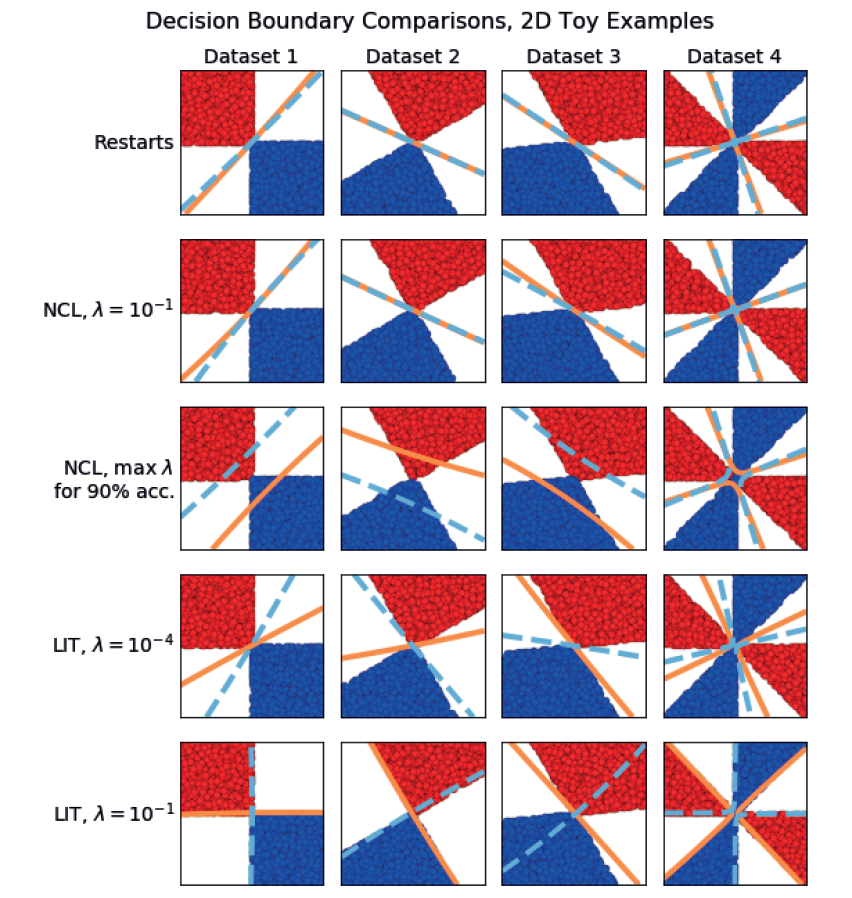
\includegraphics[width=0.75\textwidth]{dis_fig1.png}
	\caption{Test on four 2D toy data sets. Notice the success of the usual algorithms of Random Restarts and NCL,  and how they compare to $\lambda = 10^{-4}$.}
	\label{fig:1}
\end{figure}
\begin{figure}[!ht]
\centering
	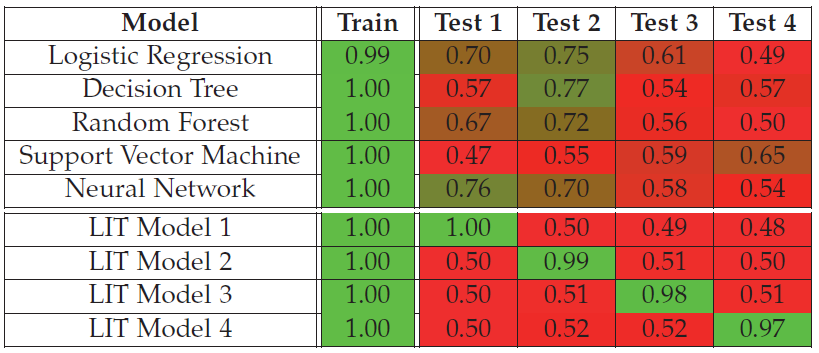
\includegraphics[width=0.75\textwidth]{dis_fig2.png}
	\caption{Testing popular machine learning models and LIT with an 8D data set with four 2D characteristics embedded. Notice that each traditional model learns a combination of all the rules, but LIT is forced to learn one model at a time.}
	\label{fig:2}
\end{figure} 

The thesis briefly proposes using gradient smoothing in adversarial neural networks to create more consistent, robust behavior. Testing an adversarial model with traditional training, gradient regularization, and a combination of adversarial and gradient regularization showed a slight increase in robustness. The degree of change was very dependent on the characteristics of the data. Some models were nearly identical, while others had an apparent deviation in behavior when the smoothing was included. Because of the inclusion of input gradients, the reader can infer a relation to the loss functions previously derived. Still, there is no apparent connection between the loss function in \cref{fn:1} and \cref{fn:3}.


%---------------------------------------------------------------------

\section{Interpretability with Human's Study}
\label{sec:explainability}
The second portion of the thesis explores a specific integration of three standard disentanglement algorithms (Ground-Truth (GT), Autoencoders (AE) \textbf{95} and Variational autoencounters (VAE) \textbf{113}) as well as three broader ``interpretable" models that do not depend on ground truths ($\beta$-TCVAE (TC)\textbf{45}, Semi-supervised $\beta$-TCVAEs (SS), and InfoGAN (IG)\textbf{46}) with an interactable, visual representation. The authors use three data sets: dSprite \textbf{158}, Sinelines, a 64-dimension data set generated off of a linear combination of a linear function and sin-wave, and MNIST \textbf{132}. MNIST was a good choice because it is the quintessential neural network problem of identifying handwritten numbers. There were two central portions of their testing, speak-aloud and quantitative metrics. The former followed a total sample of 13 individuals, divided into a 3 sample pilot and 10 sample test, taking detailed notes on the qualitative responses using the developed software. The broader test, which spanned 195 individuals (90 on dSprite and sinewaves, 105 on MNIST), measured the completion rate, response time, slider distance, correctness rate, self-reported confidence, and self-reported understanding. Their results can be seen in \cref{fig:3}. 

\begin{figure}[!ht]
\centering
	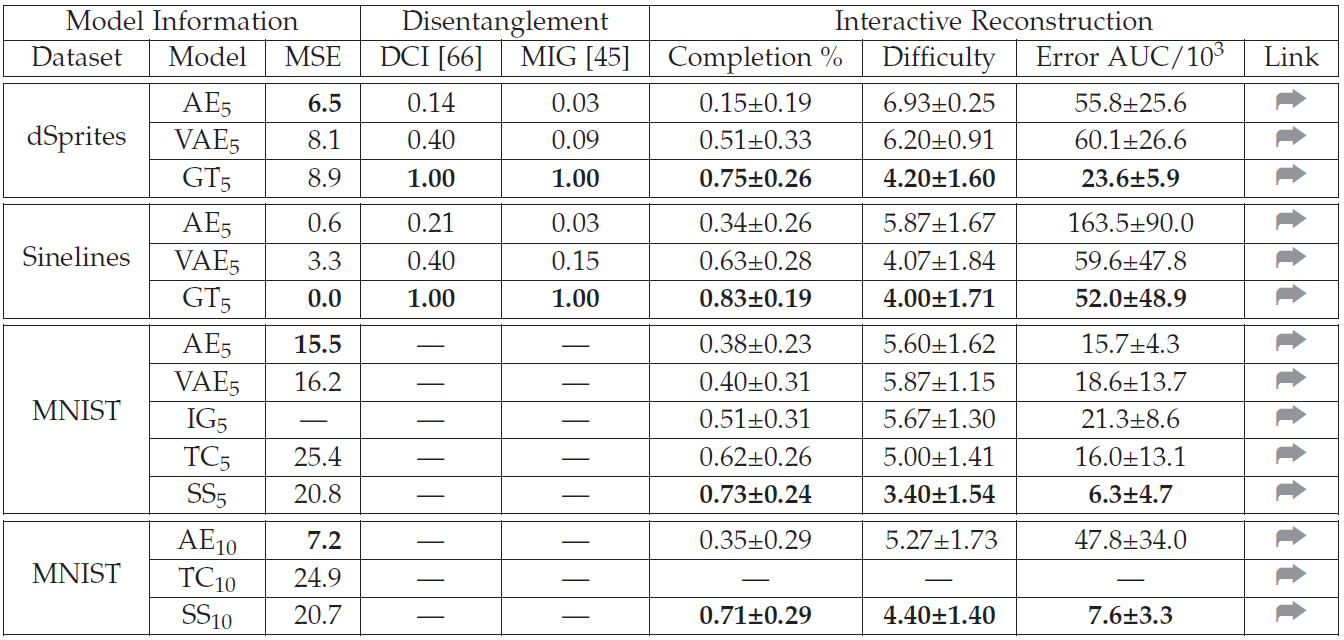
\includegraphics[width=0.95\textwidth]{dis_fig3.png}
	\caption{}
	\label{fig:3}
\end{figure}

This is my first look at a study that involved human subjects, so the analysis given should be considered with that in mind. The sample base from which the samples were taken was primarily a pool of computer science students. Using individuals potentially versed in complex computational systems, such as neural networks, could introduce another variable not considered here. The interactive representation contrasts with a ``single-dimension task," where a snapshot of a set of situations with varying input values is given. The sample is tasked with understanding each piece of information. Ross states that this model violates the motive of the interactive representation on four criteria: 1) it only presents part of the model, 2) it presents dimensions separately, 3) separates visualization from the task, and 4) it provides feedback sporadically instead of consistently. This seems to be a fundamental error in the experimental design. Four variables of the system are proposed, and all vary simultaneously. With the restriction of funding to pay for individuals to participate, the motivation is understandable. Still, when all four variables are changed, the importance of any one individual motivation can not be analyzed. It would have been better to design experiments that tested the individual, and compound, improvement each variable had on the success of the understanding task. 

The generalized result that the tests yielded was that when the model was presented in a straightforward way that could be intentionally manipulated, the subjects developed a strategy that relied on understanding each input and deducing which combination of inputs should result in the desired outcome;  this comes back to the idea of simulatibility. This is a clear demonstration of the subject evolving to a state of understanding the model. When the inputs were not effectively conveyed, the subjects resorted to an inefficient hill-climbing method paramount to random guessing. 

The topic of interpretable models is concluded with the conversation about hierarchical trees. Ross claims that this topic is ``'complementary to recent shifts in disentanglement research." By considering a causal relationship between rules, one rule being triggered causes another rule to be considered. This can be explained as a tree-type structure, where each node describes an implicit rule, which, as described earlier, explains a reason. These chains of rules represent a more abstract explanation of the decision space. Ross proposes an algorithm to derive these trees and claims that a good measure of performance is the H-error, how much the derived tree lines up with the initial ground truths, purity, how well the outputs match the ground truth, and coverage, how much of the input space the final tree covers. Initial tests of the tree show it is competitive with state-of-the-art models while providing an abstract explainability. 

%---------------------------------------------------------------------

\section{Contributions}
\label{sec:contributions}
To summarize the critical contributions of the first half of the paper: a reason-based loss function was derived to generate multiple models with unique ``reasons". This novel loss function was based on the concept of reasons being encoded as gradients and searching for locally orthogonal input gradient vectors, decreasing the impact of used gradients in subsequent models. Using toy data, this model extracts models with unique reasons and searches through the whole space, where the order depends on the reason's importance. This model was harder to analyze for complex, real-world data but did seem to extract a set of comparable models that displayed slightly different behavior, hinting at models with other reasons. The concept of input gradients was then expanded to adversarial networks to show that the higher-level idea can be used between models. It was stated that there needed to be a human subject study to analyze how well the extracted reasons represented attacks and defenses. 

The second half of the paper tackled effectively representing these interpretable models. The author defaulted to the field of disentanglement and popular methods to develop a set of models. It would have been advantageous for them to continue with the models developed in the first half and compare their algorithm results to popular methods. Through an arduous testing process, the author confirmed what intuition tells us: that allowing subjects to play with models significantly increases understanding. When those models are designed well, the play becomes more effective. The blending of think-aloud style studies and metric-based studies provides a well-rounded interpretation; however, limiting the subject pool to computer science students may introduce some fundamental biases to problem approach and initial understanding. 

Finally, the author presents a hierarchical approach to the disentanglement idea. The theoretical basis developed for decomposing disentangled reasons into a type of decision tree seems relatively sound. Several performance metrics and distance measurements are well-formed and don't act under the assumptions of universally flat topologies. This idea could have used more experimental testing to analyze the actual efficacy of the approach, but the author sets up well for a follow-up paper on the subject. 

%---------------------------------------------------------------------

\section{Conclusion}
\label{sec:conc}
Closing the gap between humans and artificial intelligence is an important topic, and this thesis grapples with a few of the many facets that describe the problem. The breadth of the focus spanned from the development of a specific loss function to the integration of interpretable representations. Because of how short the thesis was, most of the topics seemed to be weakly inspired by each other, if at all. Individually, each of the issues is well explained and serves as an essential contribution to the world of explainable artificial intelligence in some way. More care should have been taken to develop a whole project that integrates the input gradient concept into one loss function that is shown to work in the adversarial context, is utilized in an interactive, interpretable representation, and finally allows for the derivation of a hierarchical tree representation. Instead, these ideas are presented and loosely used to motivate the next topic. It would be interesting to see further work that moves to unite these four concepts into one impressive project.

%---------------------------------------------------------------------

\vskip 0.2in
\bibliography{disertation_critique}

\end{document}